\documentclass{article}
\usepackage[margin=2cm]{geometry}
\usepackage[utf8]{inputenc}
\usepackage{todo}
\usepackage{url}
\usepackage{caption}
\usepackage{subcaption}
\usepackage{graphicx}
\usepackage{listings}
\usepackage{color}
\usepackage{textcomp}
\usepackage{float}
\usepackage{amsmath}
\usepackage{tabto}

\definecolor{gainsboro}{rgb}{0.86, 0.86, 0.86}

\lstset{frame=tb,
  aboveskip=3mm,
  belowskip=3mm,
  showstringspaces=false,
  columns=flexible,
  basicstyle={\small\ttfamily},
  numbers=none,
  breaklines=true,
  breakatwhitespace=true,
  tabsize=4,
  language=C
}

\title{The World of Quantum Mechanics}
\author{Knut Andre G. Prestsveen}
\begin{document}
\maketitle


\section{Abstract}
The system with a particle in an infinite potential well, "particle in a box", is one of the simplest and most well known systems in quantum mechanics, and one of the few for which there are analytical solutions available. In this study, numerical methods for solving the Schrödinger equation are implemented, and the computed solutions for the particle box are compared against the well known analytical solutions. Going further a potential barrier is added to the box, giving rise to a tunneling phenomena, and different methods for evolving wavefunctions in time are also implemented and tested.

The computed eigenvalues and eigenstates of the empty box are found to be in good agreement with the analytical solutioins, as long as the discretization resolution is reasonably high. [...] Euler, CN, ...

\section{Introduction}
Quantum mechanics is a very extensive field in physics and chemistry, and is even applied in rather common technologies such as lasers and LEDs. Quantum mechanical problems are however very rarely analytically solveable, with the aforementioned particle in a box being an exception, and numerical routines, which is the theme of this study, are therfore necessary.

\section{Theory and method}\label{section:theory}
In quantum mechanics every system's state is completely described by a wave function, $\Psi$, and the Schödinger equation,

\begin{equation}
    i\hbar \frac{\partial}{\partial t} \Psi = \hat{H} \Psi, \quad
    \hat{H} = -\frac{\hbar}{2m} \frac{\partial^2}{\partial x^2} + V(x, t),
    \label{eq:TDSE}
\end{equation}
describes how a system's wavefunction evolves with time for some potential $V(x, t)$, and is the baseline of quantum mechanics. In equation \ref{eq:TDSE} $\hbar$ is Planck's constant and $\hat{H}$ is the Hamiltonian operator of the system.

\subsection{Dimensionless variables}
When doing numerics in general, it is usefull to work with scaled, dimensionless variables, in order to avoid having to keep track of units and getting inaccuracy errors due to the limited precision of floating point numbers. The problem is therfore rewritten with the variables $x' = x/x_0$ and $t' = t/t_0$, and since the system at hand is inside an infinite potential well, the boundery conditions on the wave functions is $\Psi(x=0) = \Psi(x=L) = 0$, and a natural choice for $x_0$ is therfore the length of the well $L$. Differentiating $Psi(x, t)$ with the chain rule and inserting into equation \ref{eq:TDSE} gives

\begin{equation}
    i\hbar \frac{\partial \Psi}{\partial t} = -\frac{\hbar^2}{2mL^2}\frac{\partial^2 \Psi}{\partial x'^2}\Rightarrow - \frac{\partial ^2 \Psi}{\partial x'^2} = i \frac{2mL^2}{\hbar}\frac{\partial \Psi}{\partial t}
\end{equation}
Now, observing that

\begin{equation}
    \left[\frac{2mL^2}{\hbar} \right] = \frac{kgm^2}{Js} = \frac{kgm^2}{s}\frac{s^2}{kgm^2}=s,
\end{equation}
we set $t_0 = \frac{2mL^2}{\hbar}$ and can then write equation \ref{eq:TDSE} with the dimensionless variables as

\begin{equation}
    -\frac{\partial^2\Psi}{\partial x'} = i\frac{\partial\Psi}{\partial t'}
\end{equation}
The system's eigen states $\psi_n$ and energy levels $E_n$ are obtained from the time independent Schrödinger equation

\begin{equation}
    \hat{H}\psi_n = E_n \psi_n
\end{equation}
which is an eigenvalue equation, and inserting the dimensionless variables results in

\begin{equation}
    -\frac{\partial ^2\psi_n}{\partial x'^2} = \lambda_n \psi_n, \quad \lambda_n = 
    \frac{2mL^2}{\hbar^2}E_n
    \label{eq:TISE-dimless}
\end{equation}
With the dimensionless variables $x' \in [0, 1]$ the boundary conditions becomes $\Psi(x'=0) = \Psi(x'=1) = 0$.

\subsection{Discretization}
To solve equation \ref{eq:TISE-dimless} we discretize the dimensionless Hamiltonian using the central difference scheme twice to approximate the second derivative, and en up with the matrix equation

\begin{equation}
    H\psi_n = \lambda_n \psi_n, \quad H_{ii} = \frac{2}{\Delta x'^2} + V_i, 
    H_{ii\pm1}=\frac{-1}{\Delta x'^2},
\end{equation}
which is solved using e.g. Lapack's ***eigh*** routine. Here $\Delta x$ is the spacing between each node in the dircetized space, and we can equivalently write $H_{ii} = 2N^2 + V_i, H_{i\pm1} = -N^2$. $N$ is the number of spacial nodes, and this latter forumaltion is how it is implemented in the code.

\subsection{Time evolution}
Time evolution, write about:
\begin{itemize}
    \item eigenfunc expansion
    \item Euler/CN
\end{itemize}

\subsection{Bound States}
\begin{itemize}
    \item num bound states
    \item root finding
\end{itemize}

\section{Results and discussion}
\subsection{Particle in an empty box}
The numerical implementation is first tested on the particle in a box problem, for which analytical solutions are well known. Figure \ref{fig:box-eigenvals} is a plot of the computed and analytical eigenvalues, and figure \ref{fig:box-eigenvals-ratio} is a plot of the ratio between them. From these figures it is easily seen that the numerical routine works very well for smaller energies, and the ratio of the computed and analytical values is about one for values lower than $200$ in this particular case with $N = 1000$ spacial nodes.

\begin{figure}[H]
    \begin{subfigure}[b]{0.5\textwidth}
        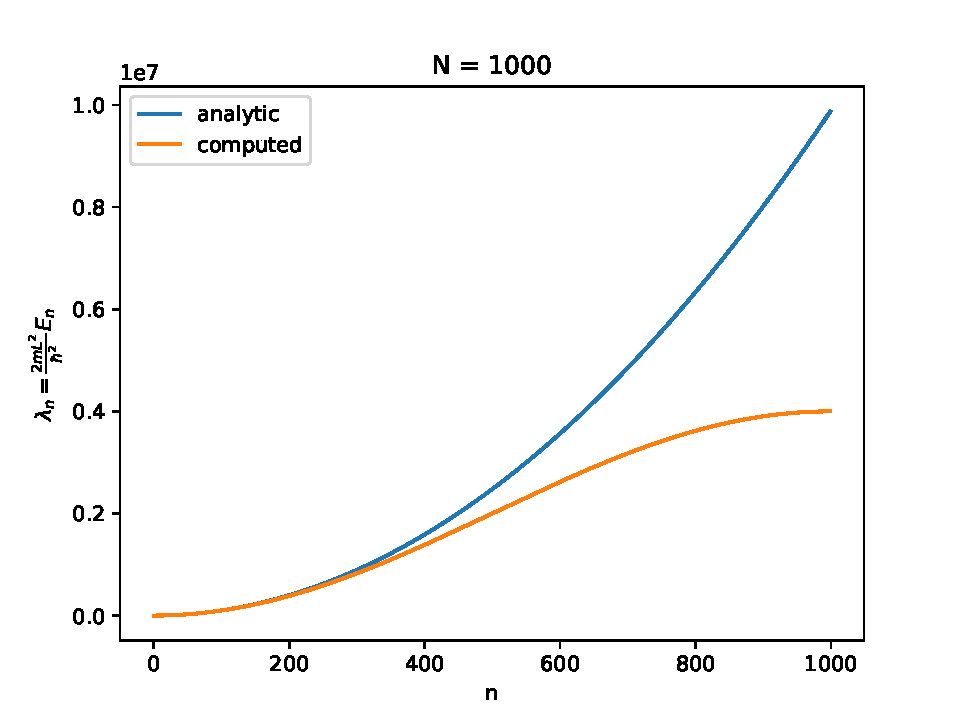
\includegraphics[width=\textwidth]{./media/eigenvalues_empty_box.pdf}
        \caption{Eigenvalues.}
        \label{fig:box-eigenvals}
    \end{subfigure}
    %
    \begin{subfigure}[b]{0.5\textwidth}
        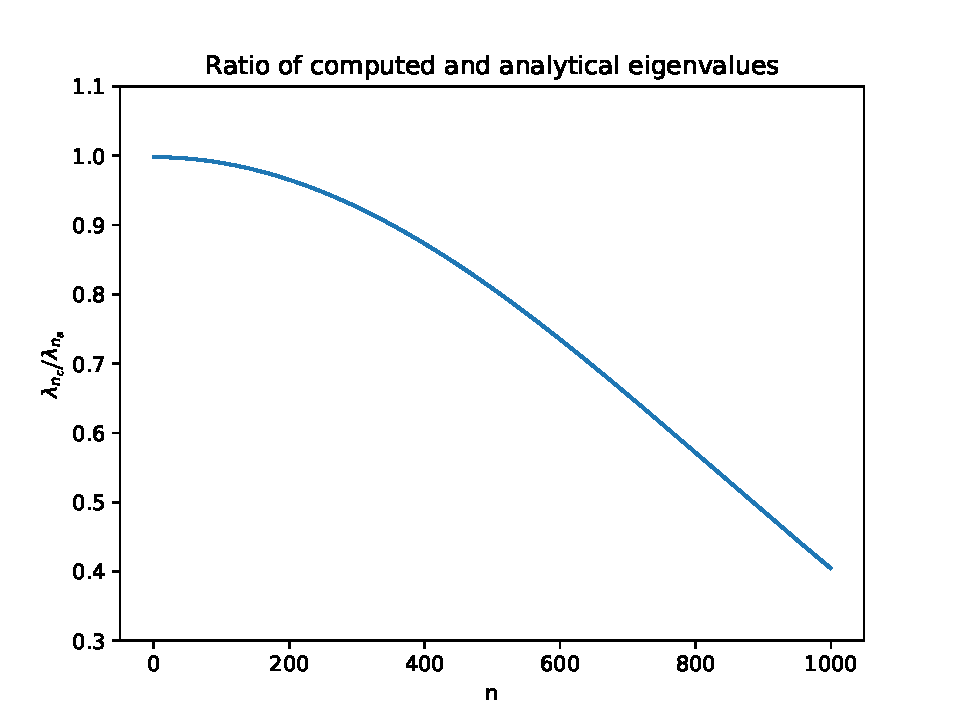
\includegraphics[width=\textwidth]{./media/eigenval_ratio_empty_box.pdf}
        \caption{Ratio - computed values over analytical.}
        \label{fig:box-eigenvals-ratio}
    \end{subfigure}
    \caption{Comparison of computed and analytical eigenvalues of the particle in a box.}
\end{figure}

Figure \ref{fig:box-eigenstates} shows the three eigenstates with the lowest energies, and the computed solutions are seemingly completely overlapping with the analytical ones. To study the accuracy of the eigenstates we use the euclidian norm of the difference between the corresponding computed and analytical solutions as a meassure of error, and figure \ref{fig:box-eigenstates-error} shows how this error scales with increasing $N$. Not surprisingly, the numerical solver seems to give better results for higher $N$.

\begin{figure}[H]
    \begin{subfigure}[b]{0.5\textwidth}
        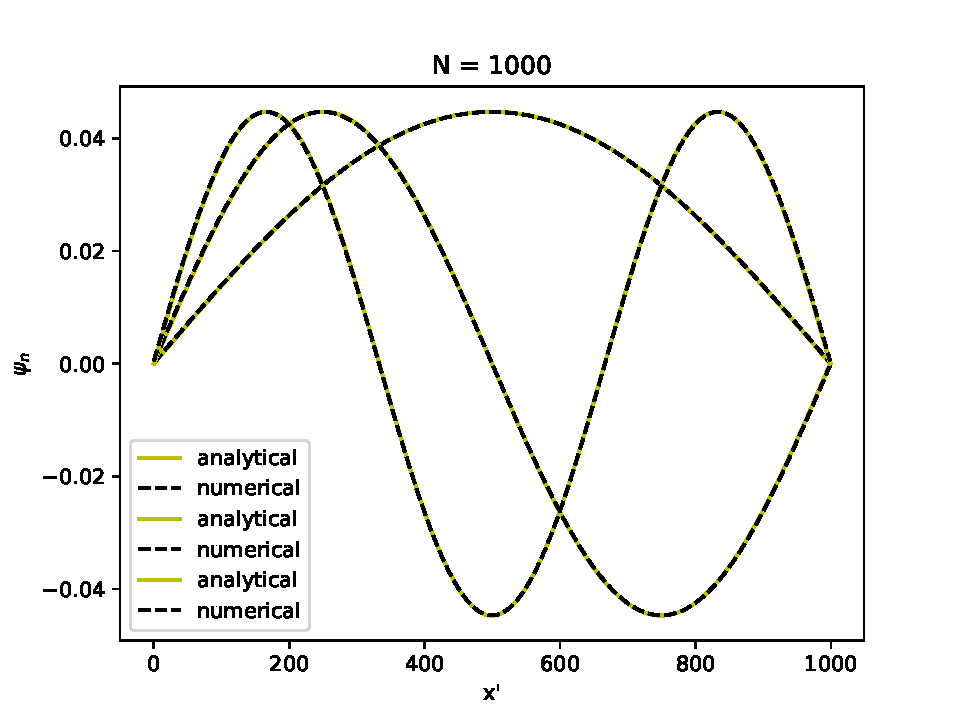
\includegraphics[width=\linewidth]{./media/eigenstates_empty_box.pdf}
        \caption{Eigenstates}
        \label{fig:box-eigenstates}
    \end{subfigure}
    %
    \begin{subfigure}[b]{0.5\textwidth}
        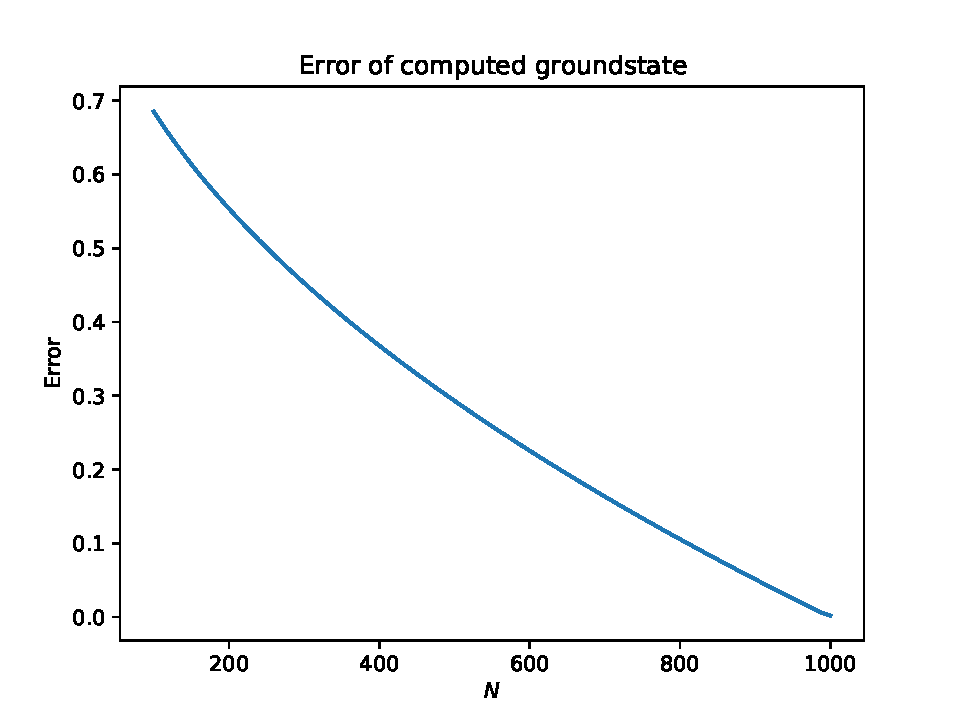
\includegraphics[width=\linewidth]{./media/wf_error_scaling.pdf}
        \caption{Error for different values of $N$.}
        \label{fig:box-eigenstates-error}
    \end{subfigure}
    \caption{Comparison of computed and analytical eigenstates of the particle in a box.}
\end{figure}

Then as a final check of our computed solutions, the orthonormality of the eigenstates is tested. The states should be orthonormal, and therfore the innerproduct between two states should be one if the states are equal, and zero otherwise, i.e.

\begin{equation}
    \langle\psi_i \mid \psi_j\rangle = \delta_{ij}.
\end{equation}
Here $\delta_{ij}$ is the Kronecker delta function. Checking the computed eigenstates we see that for $N=1000$, the maximum deviation from orthonormality, i.e. largest deviation from $0$ or $1$ is for a inner product of eigenstates, is 7.904050677853824e-15, a very small number.

\subsection{Potential well with a barrier}
After seeing the capabilities of the numerical solver, we test it on a slightly more complex system by adding a potential barrier to in the middle of the infinite well. The potential inside the well then becomes

\begin{equation}
    V(x) = 
        \begin{cases}
            V_0, & L/3 < x < 2L/3\\
            0, & \text otherwise.
        \end{cases}
\end{equation}
With the dimensionless variables we get $\nu(x') = t_0 V(x)/\hbar$, and figure \ref{fig:barrier-bound-states} shows the six bound eigenstates for this system with $\nu_0 = 1000$, i.e. the states wich eigen energies are below $V_0$.

The eigenvalues of this system can additionally be found analytically from the roots of

\begin{equation}
    f(\lambda) = e^{\kappa/3} \left[ hmm \right]^2 - 
                e^{\kappa/3} \left[ hmm \right]^2
\end{equation}
where $k=\sqrt{\lambda}$ and $\kappa=\sqrt{\nu_0 - \lambda}$. The eigenvalues $\lambda_n$ are shown in table \ref{tab:eigenvals}, from which we observe that two and two eigenvalues are almost equal. This is because there cannot be degenerate bound states in a one dimensioinal problem like this, however pairs of states being the symmetric and antisymmetric versions of the same wave are almost degenerate, with the antisymmetric state having a slightly higher energy.

\begin{tabular}{c c}
    val & val \\
    val & val \\
    val & val \\
    val & val \\
    val & val \\
    val & val \\
    \label{tab:eigenvals}
\end{tabular}

\begin{figure}[H]
    \begin{subfigure}[b]{0.5\textwidth}
        \centering
        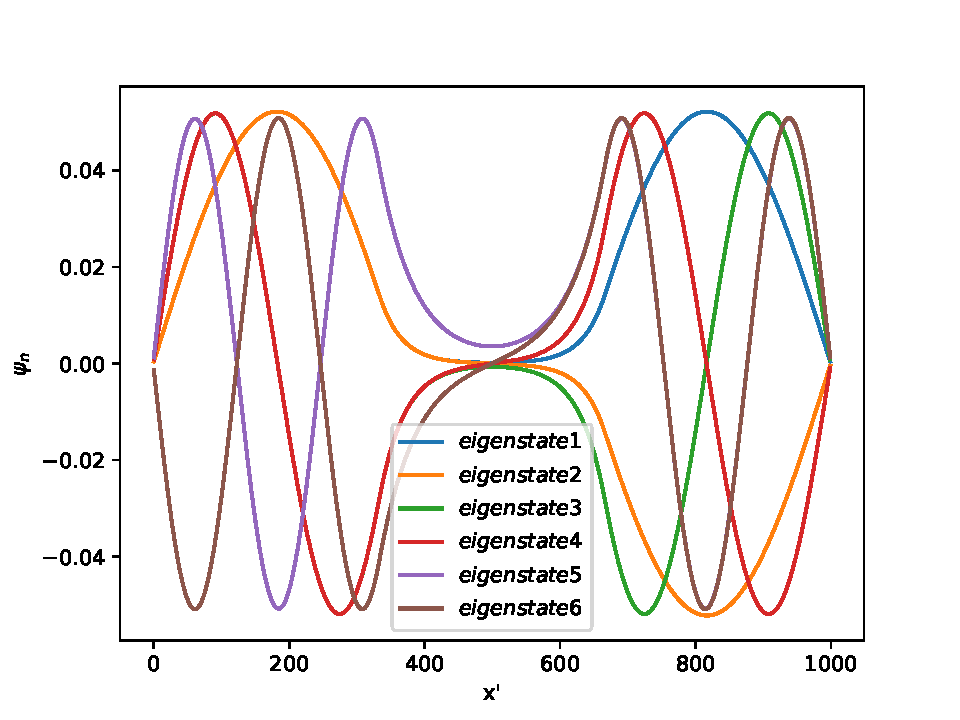
\includegraphics[width=\linewidth]{./media/bound_eigenstates_barrier.pdf}
        \caption{Barrier bound states.}
        \label{fig:barrier-bound-states}
    \end{subfigure}
    %
    \begin{subfigure}[b]{0.5\textwidth}
        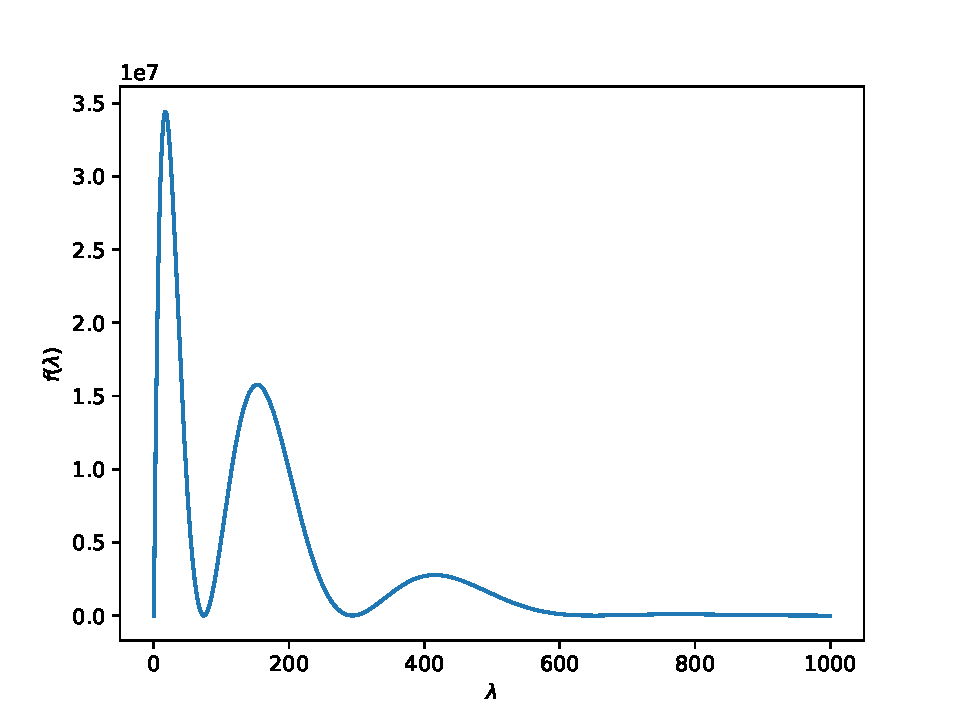
\includegraphics[width=\linewidth]{./media/f_of_lambda_roots.pdf}
        \caption{Barrier roots}
        \label{fig:barrier-roots}
    \end{subfigure}
\end{figure}

\subsection{Time evolution}
Next we study the time evolution of wave functions, by expanding the initial state in eigenstates. In figure \ref{fig:box-time-evolved1} the initial state was simply $\psi_0$, the first energy eigenstate, and in figure \ref{fig:box-time-evolved2} the initial state was the dirac delta function with the peak at $x'=1/2$, corresponding to $x = 0.5L$. Figure \ref{fig:box-time-evolved2_cn} also show the propagated delta function after the same time $t' = 0.1$, but propagated using the iterative Crank Nicolson method. Figure \ref{fig:box-time-evolved2} and \ref{fig:box-time-evolved2_cn} are both plotting what is supposed to be the same state, but they are clearly different. This could because of inaccuracy when expanding the dirac delta function in eigenstates, as it would in theory require an infinite number of eigenstates. For initial states that are difficult to write as an eigenfunction expansion, iterative methods may be better suited.

\begin{figure}[H]
    \begin{subfigure}[b]{0.5\textwidth}
        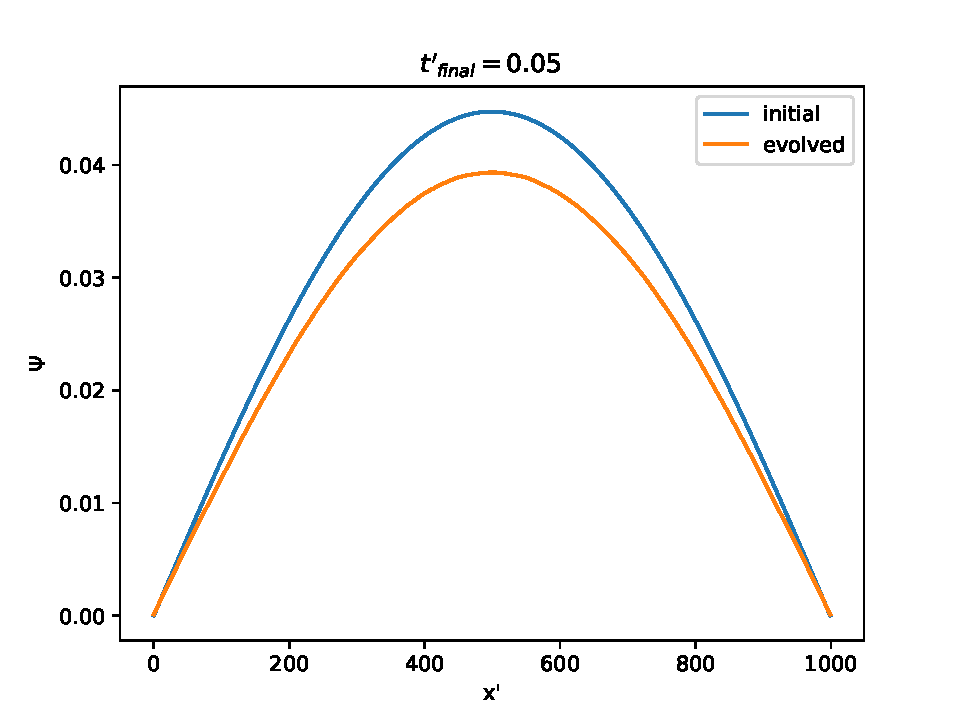
\includegraphics[width=\linewidth]{./media/time_evolve_emptybox_1.pdf}
        \caption{Empty box, time evolved eigenfunction expansion.}
        \label{fig:box-time-evolved1}
    \end{subfigure}
    %
    \begin{subfigure}[b]{0.5\textwidth}
        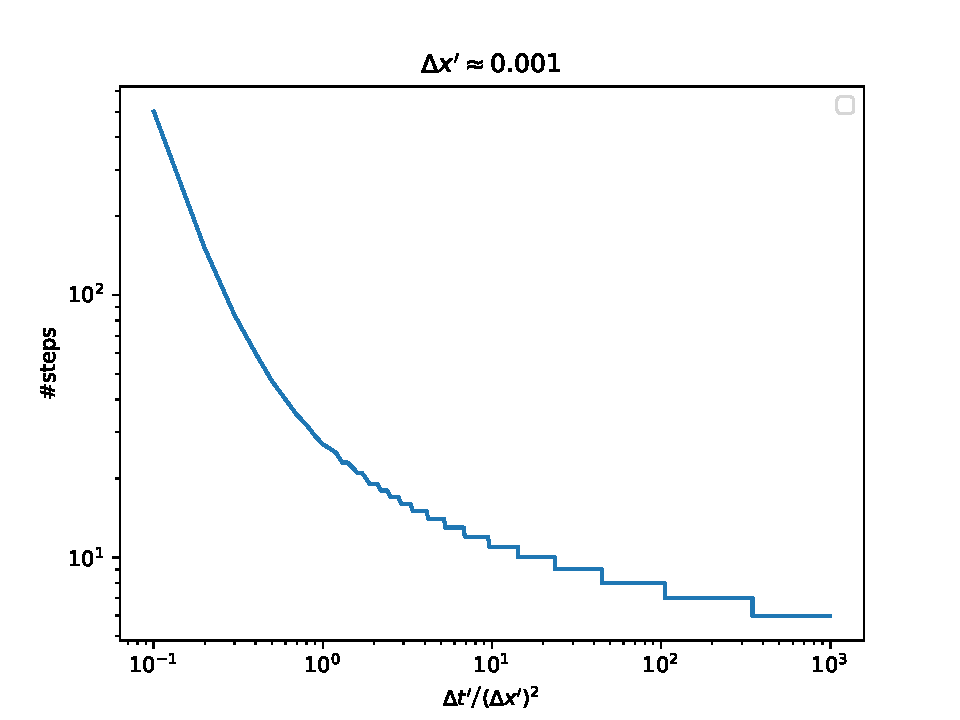
\includegraphics[width=\linewidth]{./media/steps_before_euler_collapse.pdf}
        \caption{Euler collapse}
        \label{fig:euler-collapse}
    \end{subfigure}
    %
    \begin{subfigure}[b]{0.5\textwidth}
        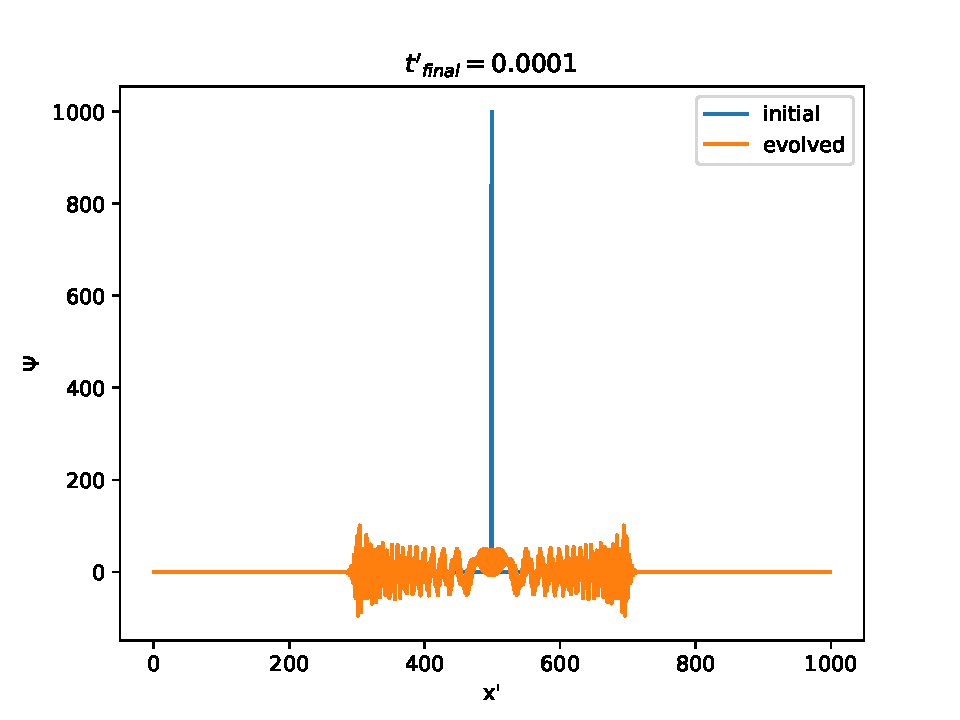
\includegraphics[width=\linewidth]{./media/time_evolve_emptybox_2.pdf}
        \caption{Empty box, time evolved eigenfunction expansion.}
        \label{fig:box-time-evolved2}
    \end{subfigure}
    %
    \begin{subfigure}[b]{0.5\textwidth}
        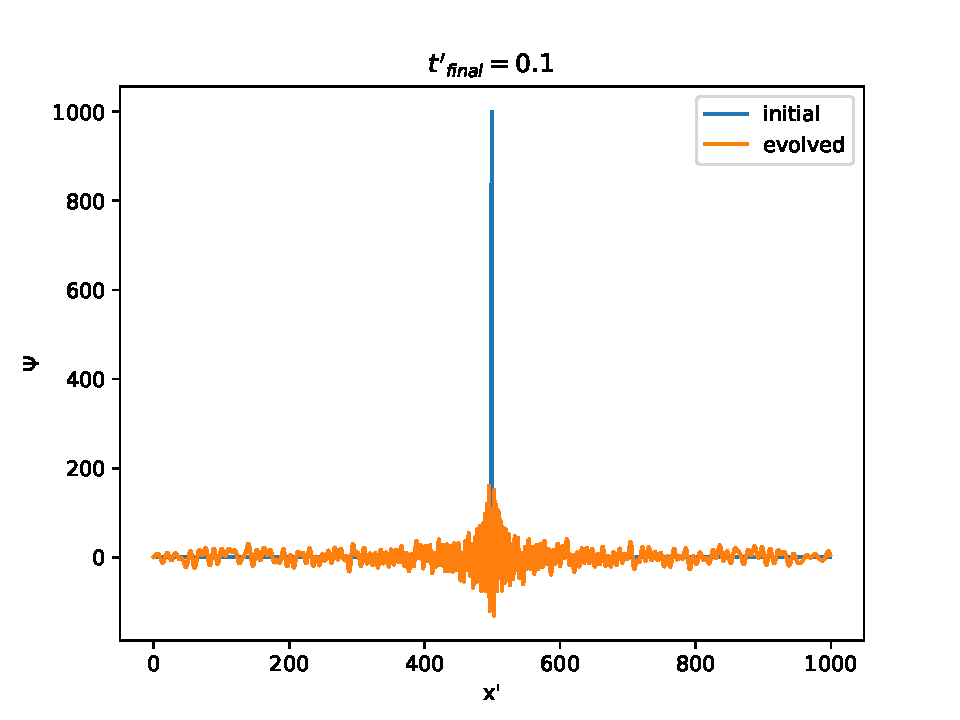
\includegraphics[width=\linewidth]{./media/time_evolve_emptybox_2_cn.pdf}
        \caption{Empty box, time evolved Crank Nicolson.}
        \label{fig:box-time-evolved2_cn}
    \end{subfigure}
    \caption{Time evolution lol}
\end{figure}

As mentioned in section \ref{section:theory}, the forward Euler scheme does not conserve probability, and will cause the computed wavefunction to break down after enough iterations. In figure \ref{fig:euler-collapse} it is shown how many iterations it takes for the Euler method to collapse as a function of Courant-Friedrichs-Lewy (CFL) number $\Delta t/\Delta x^2$. A collapse was in this case arbitrarily defined to be when the propagated wavefunction's total probability, which should always be $1$, deviated by more than $1$. This means that the wavefunction become unphysical earlier than what is indicated in \ref{fig:euler-collapse}, which only shows how it depends on the CFL number. When a wavefunction has broken down will depend on the chosen treshhold. The Crank Nicolson method does however conserve probability, and is a better, more stable routine. Figure \ref{fig:crank-nicolson} shows the same initial state propagated using this method.

Then we try to propagate a wavefunction in the barrier potential, and we let the initial state be $\Psi_0 = (1/\sqrt(2)(\psi_1 + \psi_2))$, the superpositon of the two first eigenstates, which is mainly located on one side of the barrier. The initial state is plottet in figure \ref{fig:barrier-initial-state}, and the propagated probability distribution is plotted through time in figure \ref{fig:barrier-evolve-surface}.

\begin{figure}[H]
    \begin{subfigure}[b]{0.5\textwidth}
        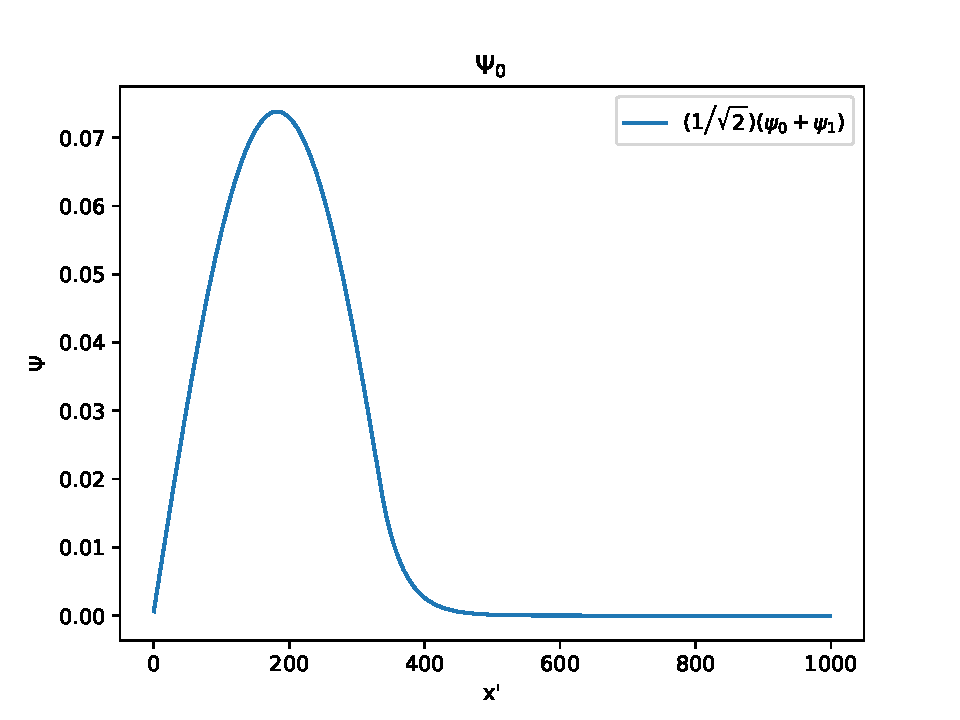
\includegraphics[width=\linewidth]{./media/initial_state.pdf}
        \caption{Barrier initial state}
        \label{fig:barrier-initial-state}
    \end{subfigure}
    %
    \begin{subfigure}[b]{0.5\textwidth}
        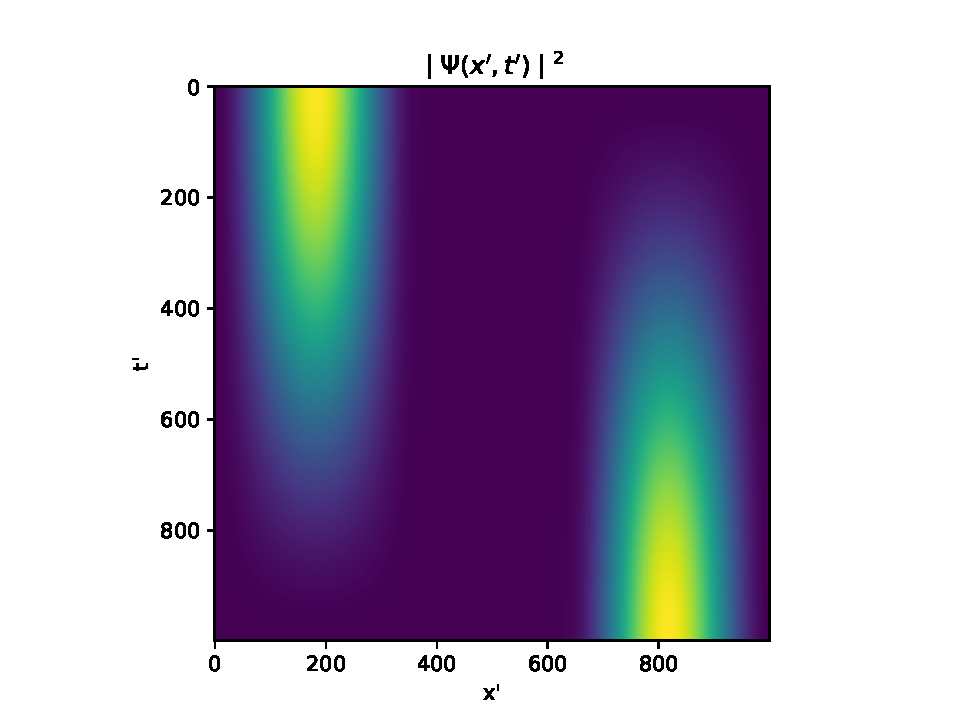
\includegraphics[width=\linewidth]{./media/time_evolve_surface.pdf}
        \caption{Barrier time evolve, surface}
        \label{fig:barrier-evolve-surface}
    \end{subfigure}
    \caption{Initial state and time propagation in the well with a potential barrier.}
\end{figure}
From figure \ref{fig:barrier-evolve-surface} we see that the probability distribution shifts from one side to the other as it propagates through time, even tough the energy of the particle is lower than the barrier height $V_0$. This is quantum tunneling, and is impossible in classical physics.


\section{Conclusion}
The numerically computed solutions for the box potential were in good agreement with the theoretical ones, this also goes for the eigenvalues of well with the barrier potential. This study therfore, while treating rather basic systems, shows that even simple numerical routines can provide great insigt in quantum mechanics such as tunneling, and quite effortlessly solve for systems that are analytically unsolvable. Going further a more thorough investigation of iterative and other methods for solving the Scrödinger equation could be a logical next step, for treating problems were the eigenfunction expansion is not suitable. This however requires a more thorough study of partial differential equations, and is beyond the scope of this paper, which is to display the use of numerics in quantum mechanics.  Ellerno

\end{document}


